\documentclass[tikz,border=6pt]{standalone}
\usepackage{amsmath,amssymb}
\usetikzlibrary{arrows.meta,calc,positioning}

\begin{document}
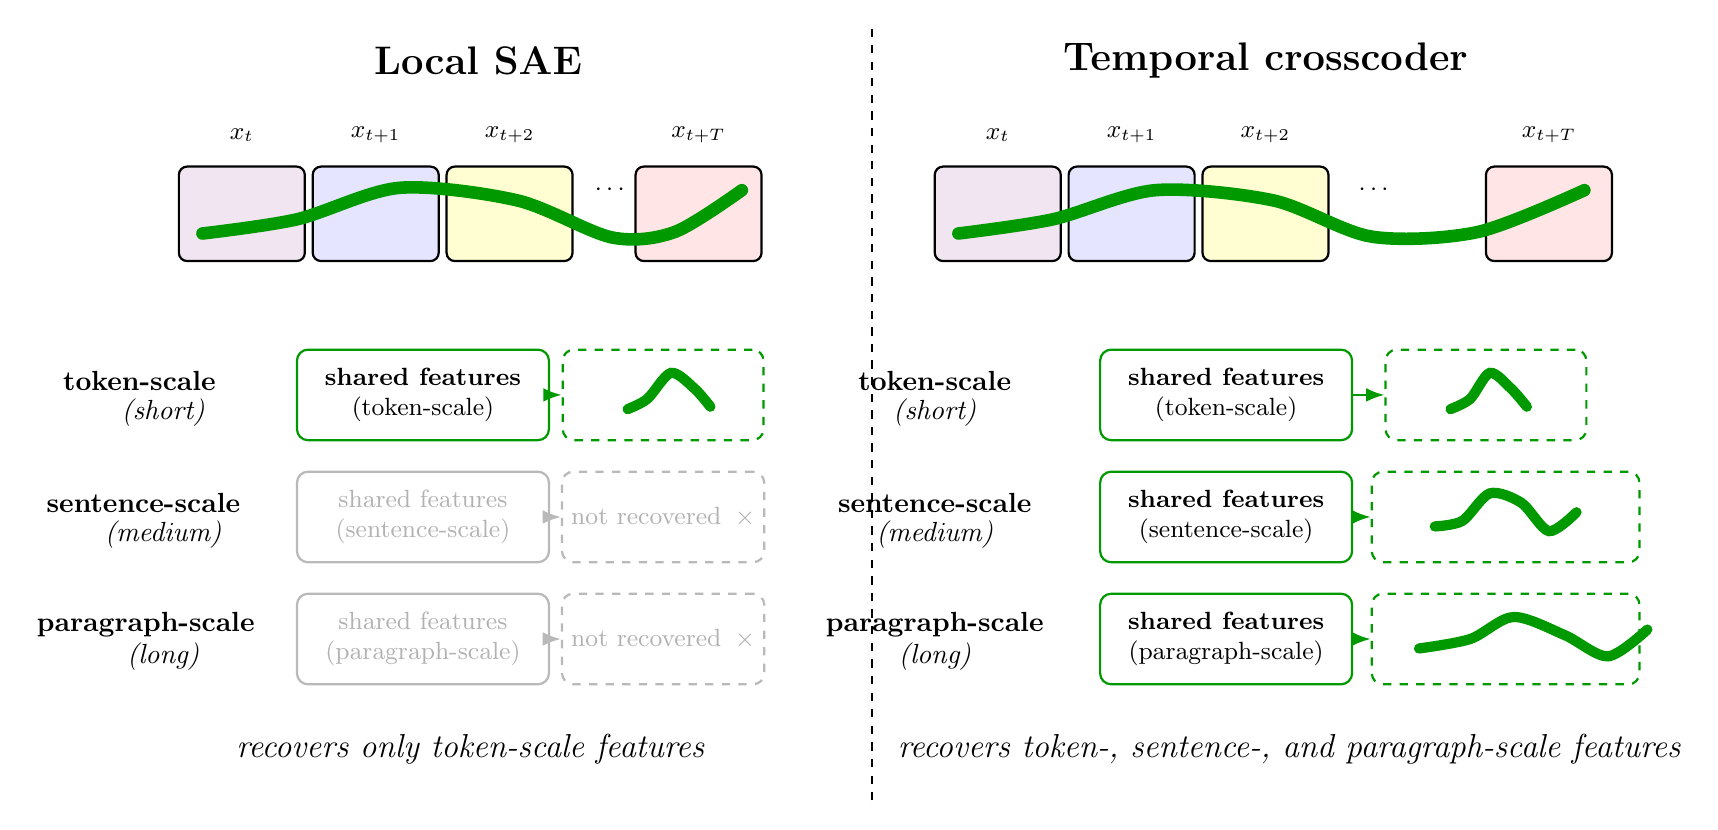
\begin{tikzpicture}[
    >=Latex,
    font=\small,
    line width=0.8pt,
    every node/.style={align=center},
    %
    tokenA/.style={draw, rounded corners=3pt, minimum width=1.6cm, minimum height=1.2cm, fill=violet!10},
    tokenB/.style={draw, rounded corners=3pt, minimum width=1.6cm, minimum height=1.2cm, fill=blue!10},
    tokenC/.style={draw, rounded corners=3pt, minimum width=1.6cm, minimum height=1.2cm, fill=yellow!18},
    tokenD/.style={draw, rounded corners=3pt, minimum width=1.6cm, minimum height=1.2cm, fill=red!10},
    %
    feat/.style={draw, rounded corners=4pt, minimum width=3.2cm, minimum height=1.15cm, fill=white, draw=green!60!black},
    featoff/.style={draw, rounded corners=4pt, minimum width=3.2cm, minimum height=1.15cm, fill=white, draw=gray!55, text=gray!60},
    %
    outbox/.style={draw, rounded corners=4pt, dashed, minimum width=2.55cm, minimum height=1.15cm, fill=white, draw=green!60!black},
    outboxlong/.style={draw, rounded corners=4pt, dashed, minimum width=3.4cm, minimum height=1.15cm, fill=white, draw=green!60!black},
    outoff/.style={draw, rounded corners=4pt, dashed, minimum width=2.55cm, minimum height=1.15cm, fill=white, draw=gray!55, text=gray!60},
    %
    scalelbl/.style={font=\bfseries},
    scaletxt/.style={font=\itshape},
    title/.style={font=\bfseries\Large},
    captiontxt/.style={font=\itshape\large},
]

% =========================================================
% Geometry constants — keep panels mirror-symmetric
% =========================================================
% Token x-positions on the LEFT panel
\def\Lxa{1.2}  \def\Lxb{2.9}  \def\Lxc{4.6}  \def\Lxdots{5.9}  \def\Lxd{7.0}
% Token x-positions on the RIGHT panel (mirror of left, panel-centered)
\def\Rxa{10.8} \def\Rxb{12.5} \def\Rxc{14.2} \def\Rxdots{15.6} \def\Rxd{17.8}
% Top-token y row, label row, scale rows
\def\ytop{3.25}  \def\ylab{4.25}
\def\ytok{0.95}  \def\ysen{-0.6}  \def\ypar{-2.15}
% Feature column centers
\def\Lfx{3.5}    \def\Rfx{13.7}
% Output column centers
\def\Lox{6.55}   \def\Rox{17.0}    \def\Roxlong{17.25}
% Curve heights match within each row
\def\curvey{3.0}

% =========================================================
% Panel titles and divider
% =========================================================
\node[title] at (4.2, 5.2) {Local SAE};
\node[title] at (14.2, 5.2) {Temporal crosscoder};
\draw[dashed] (9.2,-4.2) -- (9.2,5.6);

% =========================================================
% LEFT PANEL: top sequence
% =========================================================
\node at (\Lxa,\ylab) {$x_t$};
\node at (\Lxb,\ylab) {$x_{t+1}$};
\node at (\Lxc,\ylab) {$x_{t+2}$};
\node at (\Lxdots,\ylab-0.7) {$\cdots$};
\node at (\Lxd,\ylab) {$x_{t+T}$};

\node[tokenA] (Lx1) at (\Lxa,\ytop) {};
\node[tokenB] (Lx2) at (\Lxb,\ytop) {};
\node[tokenC] (Lx3) at (\Lxc,\ytop) {};
\node[tokenD] (Lx4) at (\Lxd,\ytop) {};

% green curve across left sequence
\draw[green!60!black, line width=1.6mm, line cap=round]
    plot[smooth] coordinates {
        (0.7,\curvey) (1.9,\curvey+0.18) (3.2,\curvey+0.58) (4.7,\curvey+0.42)
        (\Lxdots,\curvey-0.05) (6.7,\curvey+0.02) (7.55,\curvey+0.55)
    };

% =========================================================
% LEFT PANEL: scale labels
% =========================================================
\node[scalelbl] at (-0.1,\ytok+0.18) {token-scale};
\node[scaletxt] at (0.2,\ytok-0.22) {(short)};
\node[scalelbl] at (-0.05,\ysen+0.18) {sentence-scale};
\node[scaletxt] at (0.2,\ysen-0.22) {(medium)};
\node[scalelbl] at (-0.02,\ypar+0.18) {paragraph-scale};
\node[scaletxt] at (0.2,\ypar-0.22) {(long)};

% feature boxes
\node[feat]    (Lf1) at (\Lfx,\ytok) {\textbf{shared features}\\(token-scale)};
\node[featoff] (Lf2) at (\Lfx,\ysen) {shared features\\(sentence-scale)};
\node[featoff] (Lf3) at (\Lfx,\ypar) {shared features\\(paragraph-scale)};

% output boxes
\node[outbox] (Lo1) at (\Lox,\ytok) {};
\node[outoff] (Lo2) at (\Lox,\ysen) {not recovered \hspace{0.2em}$\times$};
\node[outoff] (Lo3) at (\Lox,\ypar) {not recovered \hspace{0.2em}$\times$};

% arrows: features -> output (token-scale active, others greyed dashed)
\draw[->, draw=green!60!black] (Lf1.east) -- (Lo1.west);
\draw[->, dashed, draw=gray!55]  (Lf2.east) -- (Lo2.west);
\draw[->, dashed, draw=gray!55]  (Lf3.east) -- (Lo3.west);

% short recovered curve (token-scale only)
\draw[green!60!black, line width=1.3mm, line cap=round]
    plot[smooth] coordinates {
        (\Lox-0.45,\ytok-0.18) (\Lox-0.20,\ytok-0.05) (\Lox+0.10,\ytok+0.28)
        (\Lox+0.40,\ytok+0.08) (\Lox+0.60,\ytok-0.15)
    };

% left caption
\node[captiontxt] at (4.1,-3.55) {recovers only token-scale features};

% =========================================================
% RIGHT PANEL: top sequence
% =========================================================
\node at (\Rxa,\ylab) {$x_t$};
\node at (\Rxb,\ylab) {$x_{t+1}$};
\node at (\Rxc,\ylab) {$x_{t+2}$};
\node at (\Rxdots,\ylab-0.7) {$\cdots$};
\node at (\Rxd,\ylab) {$x_{t+T}$};

\node[tokenA] (Rx1) at (\Rxa,\ytop) {};
\node[tokenB] (Rx2) at (\Rxb,\ytop) {};
\node[tokenC] (Rx3) at (\Rxc,\ytop) {};
\node[tokenD] (Rx4) at (\Rxd,\ytop) {};

% green curve mirrors the left panel
\draw[green!60!black, line width=1.6mm, line cap=round]
    plot[smooth] coordinates {
        (10.3,\curvey) (11.5,\curvey+0.18) (12.8,\curvey+0.55) (14.3,\curvey+0.42)
        (\Rxdots-0.05,\curvey-0.04) (16.9,\curvey+0.02) (18.25,\curvey+0.55)
    };

% =========================================================
% RIGHT PANEL: scale labels
% =========================================================
\node[scalelbl] at (10.0,\ytok+0.18) {token-scale};
\node[scaletxt] at (10.0,\ytok-0.22) {(short)};
\node[scalelbl] at (10.0,\ysen+0.18) {sentence-scale};
\node[scaletxt] at (10.0,\ysen-0.22) {(medium)};
\node[scalelbl] at (10.0,\ypar+0.18) {paragraph-scale};
\node[scaletxt] at (10.0,\ypar-0.22) {(long)};

% feature boxes (all active in temporal crosscoder)
\node[feat] (Rf1) at (\Rfx,\ytok) {\textbf{shared features}\\(token-scale)};
\node[feat] (Rf2) at (\Rfx,\ysen) {\textbf{shared features}\\(sentence-scale)};
\node[feat] (Rf3) at (\Rfx,\ypar) {\textbf{shared features}\\(paragraph-scale)};

% output boxes — sentence/paragraph wider to fit longer recovered signal
\node[outbox]     (Ro1) at (\Rox,\ytok) {};
\node[outboxlong] (Ro2) at (\Roxlong,\ysen) {};
\node[outboxlong] (Ro3) at (\Roxlong,\ypar) {};

% arrows: features -> output (all three active)
\draw[->, draw=green!60!black] (Rf1.east) -- (Ro1.west);
\draw[->, draw=green!60!black] (Rf2.east) -- (Ro2.west);
\draw[->, draw=green!60!black] (Rf3.east) -- (Ro3.west);

% recovered curves at each scale
\draw[green!60!black, line width=1.3mm, line cap=round]
    plot[smooth] coordinates {
        (\Rox-0.45,\ytok-0.18) (\Rox-0.20,\ytok-0.05) (\Rox+0.05,\ytok+0.28)
        (\Rox+0.32,\ytok+0.08) (\Rox+0.52,\ytok-0.15)
    };
\draw[green!60!black, line width=1.3mm, line cap=round]
    plot[smooth] coordinates {
        (16.35,\ysen-0.12) (16.7,\ysen-0.05) (17.05,\ysen+0.30)
        (17.45,\ysen+0.18) (17.80,\ysen-0.18) (18.15,\ysen+0.06)
    };
\draw[green!60!black, line width=1.3mm, line cap=round]
    plot[smooth] coordinates {
        (16.15,\ypar-0.12) (16.80,\ypar+0.00) (17.35,\ypar+0.28)
        (18.00,\ypar+0.05) (18.55,\ypar-0.22) (19.05,\ypar+0.12)
    };

% bottom caption
\node[captiontxt] at (14.5,-3.55)
    {recovers token-, sentence-, and paragraph-scale features};

\end{tikzpicture}
\end{document}
